\documentclass[a4paper,12pt]{article}
\usepackage[verbose,a4paper,tmargin=2cm,bmargin=3cm,lmargin=2cm,rmargin=2cm]{geometry}
\usepackage[utf8]{inputenc}
\usepackage{caption}
\usepackage{graphicx}
\usepackage[polish]{babel}
\title{Kompo - sprawko}
\author{Patryk Lisik}
\date{June 2018}

\begin{document}

\begin{titlepage}
\vspace{10cm}


\centering
{\center\huge\ Programowanie komponentowe \par}
\vspace{1.5cm}
{\center\huge\bfseries Sprawozdanie z pracy projektowej  \par}
\vspace{1.5cm}
{\center\huge\bfseries Kalendarz}

\vspace{6cm}


\begin{flushright}
\begin{tabular}{lll}
Patryk & Lisik & 210254 \\ 
Dominika & Wójcik  & 210355 \\ 
\end{tabular} 
\end{flushright}

\vspace{5cm}

\begin{center}
\textbf{Infromatyka, sem IV \\}
\textbf{2017/2018}
\end{center}
 

\end{titlepage}

Stworzona aplikacja jest kalendarzem przechowującym, wydarzenia, kontakty oraz powiadomienia. Pozwala utrwalać oraz pobierać dane za pomocą formatu XML, serializacji binarnej Javy oraz bazy danych MySQL. Użytkownikowi zostaje udostępniony interfejs graficzny zaprezentowany w podpunktach 3.2.1 -  3.2.3. 
       
\section{Najważniejsze klasy warstwy danych projektu}
Warstwa danych umożliwia przechowywanie danyh o osobach wydarzeniach i powiadomieniach. Osoby są reprezentowane przez klasę Person posiadające dwa pola imię i nazwisko będące stringami. Wydarzenie jest reprezentowane poprzez klasę Event, na którą składają się opis, data początku, końca oraz lista powiadomień. Powiadomienie jest reprezentowane przez klasę Notafication, na którą składają się opis powiadomienia oraz jego data. 
Warstwa danych przechowuje wyżej wymienione obiekty. 

\begin{minipage}{\textwidth}

    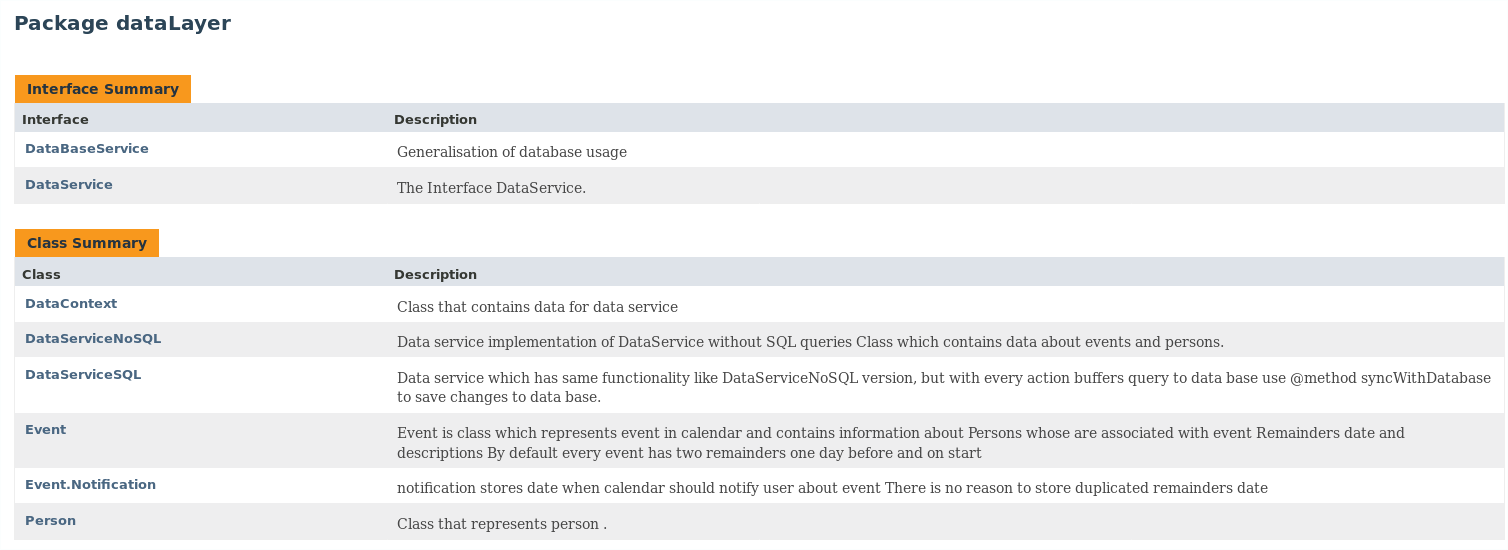
\includegraphics[width=\textwidth]{./screen/dataLayer/PackageDataLayer.png}
        \captionof{figure}{Dokumentacja package'u dataLayer}
    \label{dataLayer_pkg}

\end{minipage}

\begin{minipage}{\textwidth}

    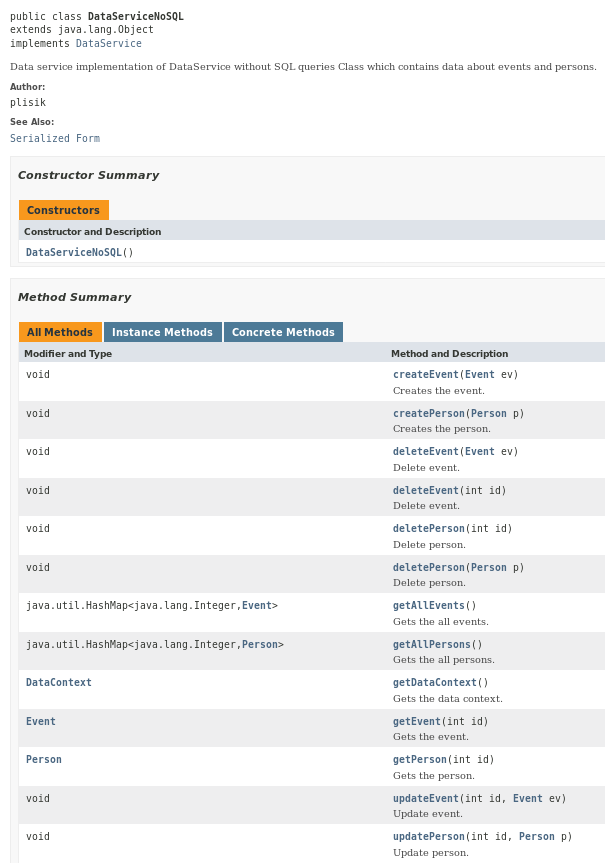
\includegraphics[width=\textwidth]{./screen/dataLayer/DataServiceNoSQL.png}
        \captionof{figure}{Dokumentacja klasy DataServiceNoSQL}
    \label{DataServiceNoSQL}

\end{minipage}

\begin{minipage}{\textwidth}

    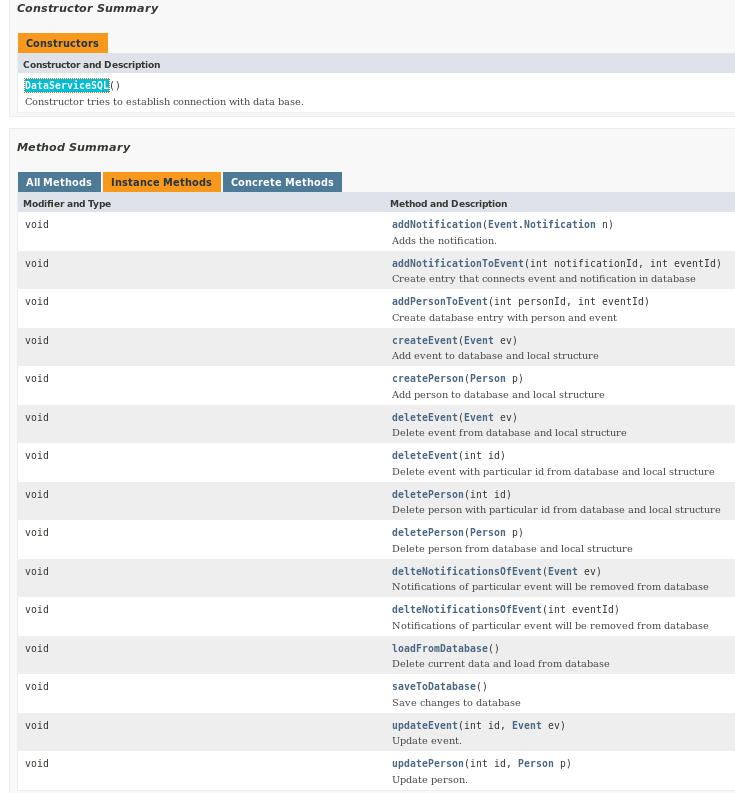
\includegraphics[width=\textwidth]{./screen/dataLayer/DataServiceSQL.png}
        \captionof{figure}{Dokumentacja klasy DataServiceSQL}
    \label{DataServiceSQL}

\end{minipage}

\begin{minipage}{\textwidth}

    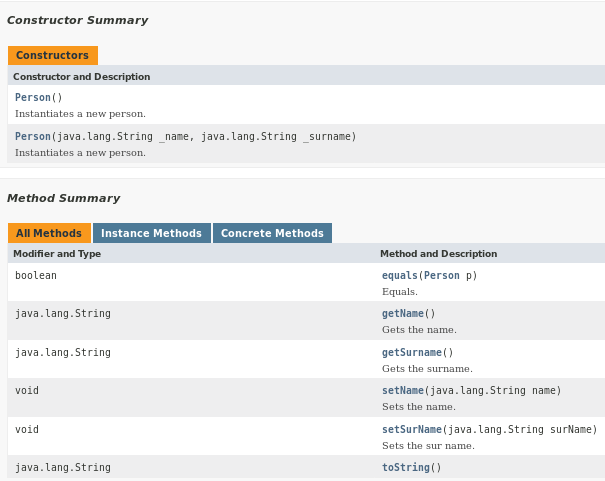
\includegraphics[width=\textwidth]{./screen/dataLayer/Person.png}
        \captionof{figure}{Dokumentacja klasy Person}
    \label{Person}

\end{minipage}

\begin{minipage}{\textwidth}

    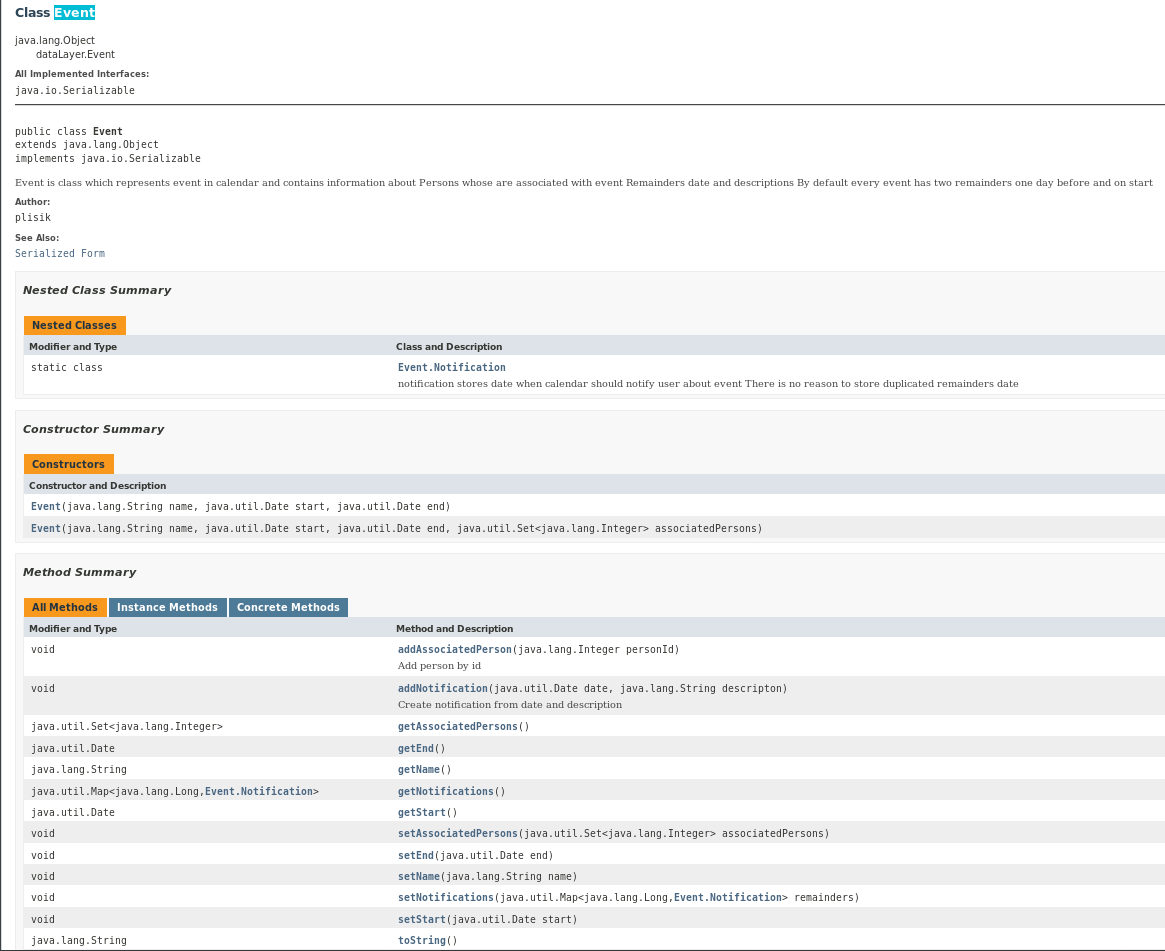
\includegraphics[width=\textwidth]{./screen/dataLayer/Event.png}
        \captionof{figure}{Dokumentacja klasy Event}
    \label{Event}

\end{minipage}


\section{Najważniejsze klasy warstwy logiki}
       Warstwa logiki umożliwia manipulowanie warstwą danych. Poza tworzeniem obiektów warstwy danych warstwa logiki umożliwia:
\begin{enumerate}
 \item znalezienie wydarzeń między datami
 \item znalezienie wydarzeń w danym dniu
 \item posortowanie wydarzeń po dacie 
 \item posortowanie wydarzeń po ilości uczestniczących osób
 \item zapis i odczyt z XML i serializacji binarnej 
\end{enumerate}

\begin{minipage}{\textwidth}

    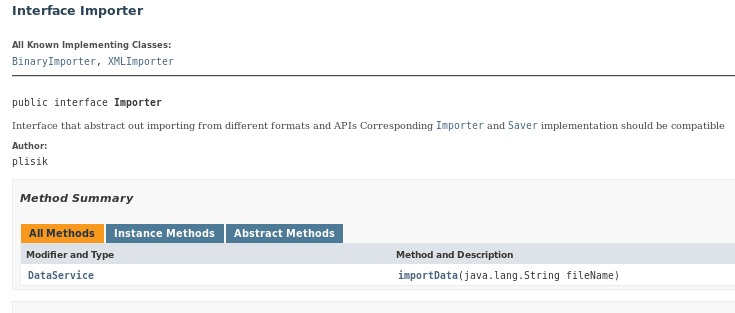
\includegraphics[width=\textwidth]{./screen/logicLayer/Importer.png}
        \captionof{figure}{Dokumentacja interfac'u Importer}
    \label{Importer}

\end{minipage}

\begin{minipage}{\textwidth}

    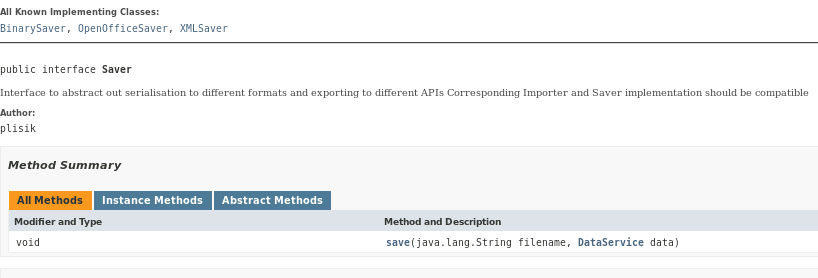
\includegraphics[width=\textwidth]{./screen/logicLayer/Saver.png}
        \captionof{figure}{Dokumentacja interfac'u Saver}
    \label{Saver}

\end{minipage}

\begin{minipage}{0.8\textwidth}

    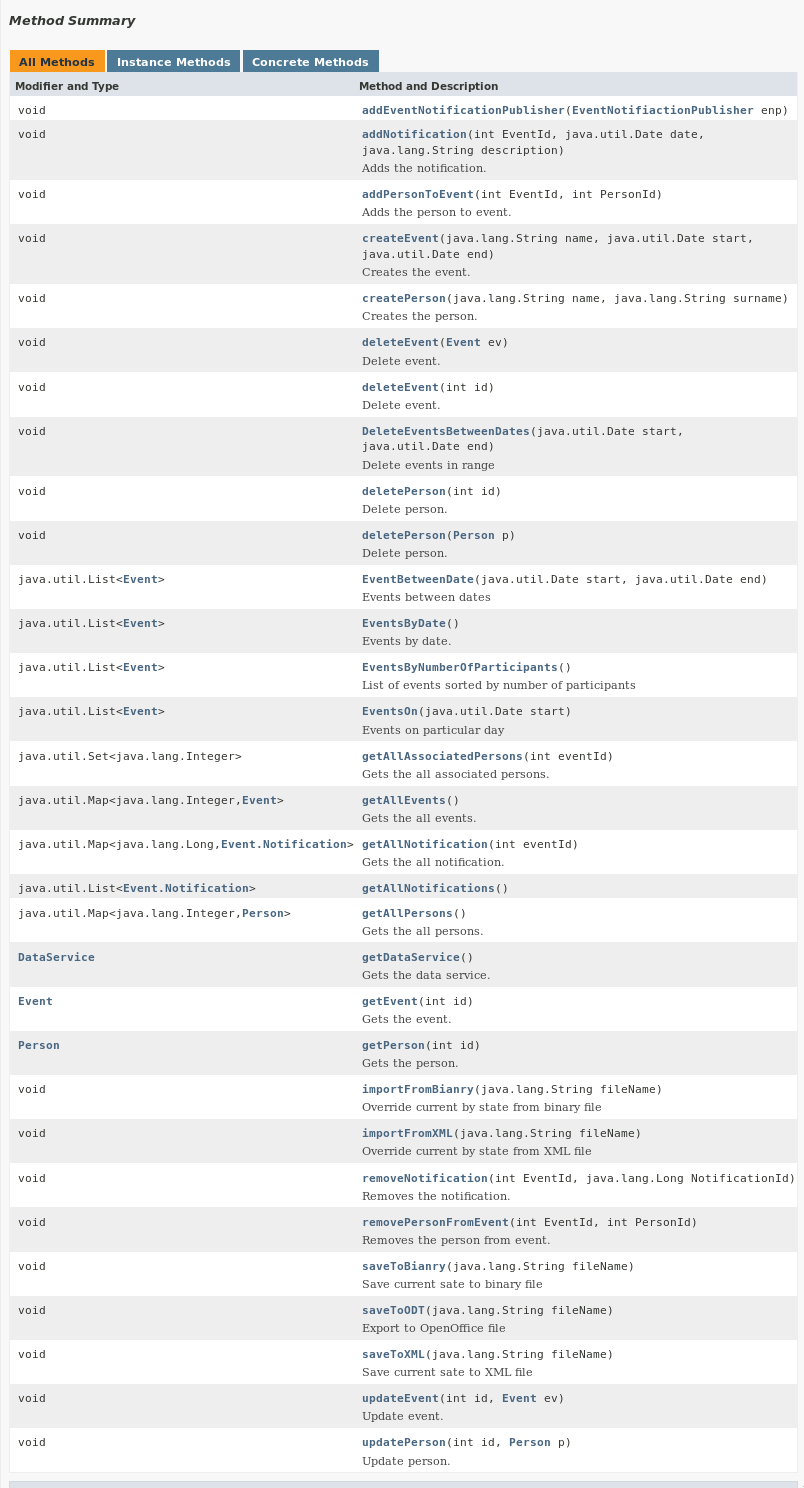
\includegraphics[width=\textwidth]{./screen/logicLayer/LogicLayerImpl.png}
        \captionof{figure}{Dokumentacja klasy LogicLayerImpl}
    \label{LogicLayerImpl}

\end{minipage}

\begin{minipage}{\textwidth}

    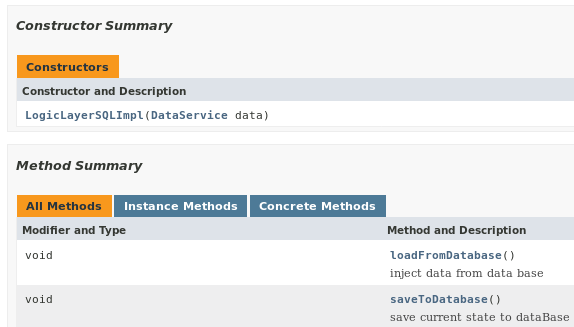
\includegraphics[width=\textwidth]{./screen/logicLayer/LogicLayerSQLImpl.png}
        \captionof{figure}{Dokumentacja klasy LogicLayerSQLImpl}
    \label{LogicLayerSQLImpl}

\end{minipage}

\begin{minipage}{\textwidth}

    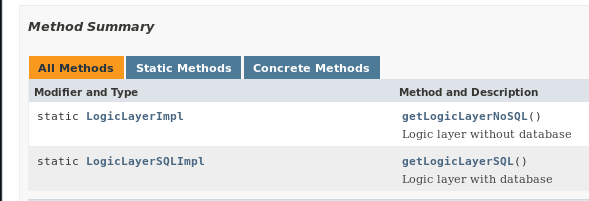
\includegraphics[width=\textwidth]{./screen/logicLayer/LogicLayerFactory.png}
        \captionof{figure}{Dokumentacja klasy LogicLayerFactory}
    \label{LogicLayerFactory}

\end{minipage}

\begin{minipage}{\textwidth}

    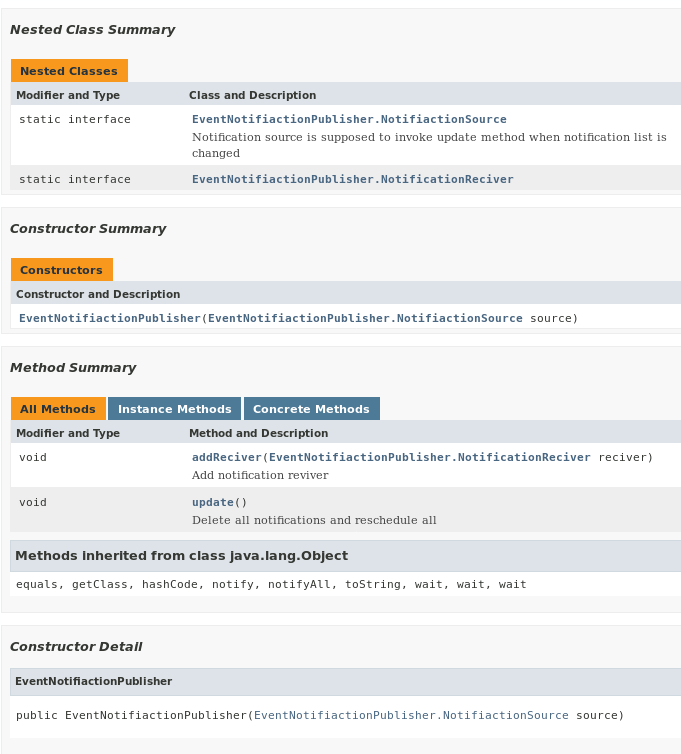
\includegraphics[width=\textwidth]{./screen/logicLayer/EventNotificationPublisher.png}
        \captionof{figure}{Dokumentacja klasy EventNotificationPublisher}
    \label{LogicLayerFactory}

\end{minipage}

\section{Warstwa interfejsu}
\subsection{Najważniejsze klasy warstwy interfejsu}
\subsection{Zrzuty ekranu najważniejszych widoków działającej aplikacji}
\subsubsection{Główne okno kalendarza ''organizera''}
\subsubsection{Okienko ''O programie''}
\subsubsection{Okienka dialogowe zapisujące/odczytujące dane i ustawienia do/z bazy/pliku XML}
\subsection{Jasny i czytelny opis klawiszy funkcyjnych i przycisków obsługujących aplikację}
\section{Postać bazy danych z zapisanymi informacjami o zdarzeniach}
\section{Podsumowanie i ewentualne uwagi grupy nt. projektu. }

\end{document}
